\chapter{Lösungsansätze für Vier Gewinnt}

\section{Optimale Strategien}
Die Analyse von 4Gewinnt aus der Perspektive der Spieltheorie zeigt eine Reihe von strategischen Prinzipien und optimalen Spielweisen um gezielte Strategien zu entwickeln. Diese Erkenntnisse beruhen sowohl auf grundlegenden Prinzipien, welche in Kapitel 3 aufgearbeitet wurden, als auch auf fortgeschrittenen Taktiken, die im Verlauf des Spiels entscheidend sein können.

Ein wichtiges Grundprinzip ist die Bedeutung des ersten Zuges. Es wurde festgestellt, dass der erste Spieler, wenn er perfekt spielt, immer gewinnen kann – vorausgesetzt, er wählt den besten Eröffnungszug. Der optimale Zug ist dabei, den ersten Stein in die Mitte zu setzen. Diese Eröffnung ermöglicht die beste Kontrolle über das Spielbrett und eröffnet viele Möglichkeiten für offensive und defensive Züge. Zieht der erste Spieler jedoch in eine der angrenzenden Spalten, führen beide Spieler bei optimalem Spiel zu einem Unentschieden. Alle anderen Eröffnungszüge gelten als weniger effektiv und führen, wenn der Gegner ebenfalls perfekt spielt, unweigerlich zur Niederlage des ersten Spielers.

Ein weiteres zentrales Prinzip ist die Kontrolle des Zentrums, die eine entscheidende Rolle spielt. Die Kontrolle über die mittleren drei Spalten (insbesondere c, d und e) ist strategisch besonders wichtig, da sie die besten Chancen für horizontale, vertikale und diagonale Gewinnreihen bietet. Auch die Spalten b und f – die zweite und vorletzte Spalte – sind wichtig, denn ohne sie kann der Spieler keine vollständigen diagonalen oder horizontalen Viererreihen bilden. Diese Kontrolle hilft nicht nur beim eigenen Spielaufbau, sondern schränkt auch die Möglichkeiten des Gegners ein.

Im Laufe des Spiels kommen zudem fortgeschrittene taktische Elemente ins Spiel. Eine wichtige Taktik ist die Schaffung von Zugzwang-Situationen, in denen der Gegner gezwungen wird, einen Zug zu machen, der seine eigene Position schwächt. Diese Situationen sind besonders am Ende des Spiels von Bedeutung, wenn nur noch wenige Felder zur Verfügung stehen und der Druck auf beide Spieler steigt. Eine weitere wichtige Taktik sind Fallenkombinationen, bei denen der Gegner durch clevere Kombinationen von Bedrohungen in eine Falle gelockt wird. Besonders wirkungsvoll sind Doppelfallen, bei denen zwei gleichzeitige Drohungen entstehen, die der Gegner nicht gleichzeitig abwehren kann. Auch Auffüllfallen sind relevant: Hier zwingt ein Spieler den Gegner durch einen Mangel an freien Feldern dazu, einen entscheidenden Stein in eine vorbereitete Blockade zu setzen.

Die spieltheoretische Analyse von „Vier Gewinnt“ wurde durch mathematische und computerbasierte Methoden weiter vertieft. Unabhängig voneinander fanden zwei Forscher eine vollständige Lösung für das Spiel. Victor Allis entwickelte 1988 einen speziellen Regelsatz zur systematischen Analyse, während James D. Allen 1990 Computerprogramme einsetzte, um das Spiel vollständig zu berechnen. Beide kamen unabhängig zum gleichen Schluss: Der erste Spieler kann bei optimalem Spiel und einer Eröffnung in der Mitte immer gewinnen. Diese Erkenntnis hat nicht nur wissenschaftliche Bedeutung, sondern bildet auch die Basis für die Entwicklung von Algorithmen, die in Computerprogrammen oder Robotersystemen verwendet werden, um das Spiel optimal zu spielen. \autocites{wikipedia_vier_gewinnt}

	
	\subsection*{Mögliche Startpositionen und Spielausgänge}
	
	\textbf{1. Startposition 4 (mittlere Spalte)}
	Wenn der erste Spieler in die mittlere Spalte setzt, hat er einen nachgewiesenen Vorteil und kann bei perfektem Spiel gewinnen. Diese Eröffnung maximiert die Kontrolle über das Spielfeld.

\begin{figure}[H]
	\centering
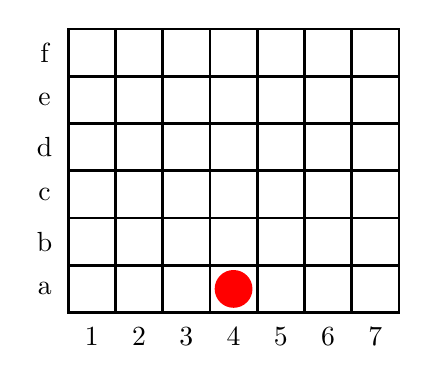
\begin{tikzpicture}[scale=0.6]
	% Zeichne das Gitter mit einheitlicher Linienstärke
	\foreach \x in {0,1,2,3,4,5,6} {
		\foreach \y in {0,1,2,3,4,5} {
			\draw[line width=1pt] (\x,\y) rectangle ++(1,1);
		}
	}
	
	% Beschriftung für Spalten (a-g)
	\foreach \x [count=\i from 1] in {1,2,3,4,5,6,7} {
		\node at (\i-0.5,-0.5) {\x};
	}
	
	% Beschriftung für Zeilen (1-6)
	\foreach \y [count=\j from 1] in {a,b,c,d,e,f} {
		\node at (-0.5,\j-0.5) {\y};
	}
	
	% Roter Stein in Feld d1 (Spalte d = 4, Zeile 1 = 0)
	\fill[red] (3.5,0.5) circle(0.4);
\end{tikzpicture}
  \caption{ROT gewinnt bei optimalen Spiel}
\label{fig:connect4_example}
\end{figure}

	
	
	\textbf{2. Startpositionen 3 oder 5 (benachbarte Spalten zur Mitte)}
	Ein Zug in die Spalte 3 oder 5 führt bei optimalem Spiel zu einem Remis, da der zweite Spieler durch eine Kombination aus Zentrums- und Blockstrategien den Sieg verhindern kann.
	
\begin{figure}[H]
	\centering
	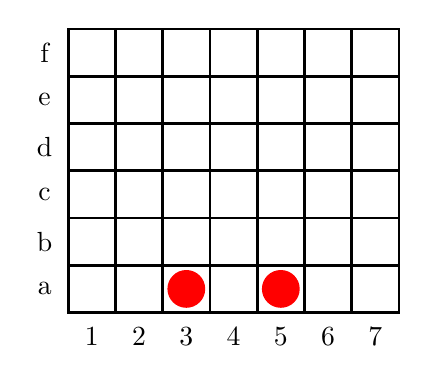
\begin{tikzpicture}[scale=0.6]
		% Zeichne das Gitter mit einheitlicher Linienstärke
		\foreach \x in {0,1,2,3,4,5,6} {
			\foreach \y in {0,1,2,3,4,5} {
				\draw[line width=1pt] (\x,\y) rectangle ++(1,1);
			}
		}
		
		% Beschriftung für Spalten (a-g)
		\foreach \x [count=\i from 1] in {1,2,3,4,5,6,7} {
			\node at (\i-0.5,-0.5) {\x};
		}
		
		% Beschriftung für Zeilen (1-6)
		\foreach \y [count=\j from 1] in {a,b,c,d,e,f} {
			\node at (-0.5,\j-0.5) {\y};
		}
		
		% Roter Stein in Feld d1 (Spalte d = 4, Zeile 1 = 0)
		\fill[red] (2.5,0.5) circle(0.4);
		\fill[red] (4.5,0.5) circle(0.4);
	\end{tikzpicture}
	\caption{Remis bei optimalen Spiel}
\end{figure}
	
	\textbf{3. Startpositionen 1, 2, 6 oder 7 (äußere Spalten)}
	Züge in die äußeren Spalten gelten als suboptimal. Der erste Spieler verliert bei perfektem Gegenspiel des zweiten Spielers, da diese Positionen weniger Kontrolle über das Zentrum und die Gewinnlinien bieten.
	
	\begin{figure}[H]
		\centering
		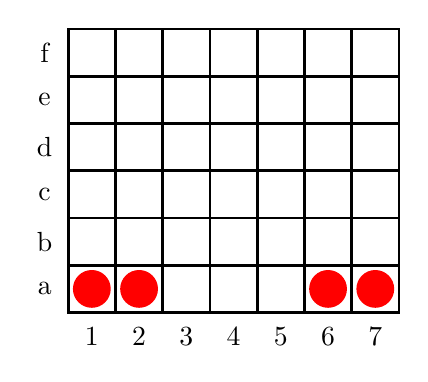
\begin{tikzpicture}[scale=0.6]
			% Zeichne das Gitter mit einheitlicher Linienstärke
			\foreach \x in {0,1,2,3,4,5,6} {
				\foreach \y in {0,1,2,3,4,5} {
					\draw[line width=1pt] (\x,\y) rectangle ++(1,1);
				}
			}
			
			% Beschriftung für Spalten (a-g)
			\foreach \x [count=\i from 1] in {1,2,3,4,5,6,7} {
				\node at (\i-0.5,-0.5) {\x};
			}
			
			% Beschriftung für Zeilen (1-6)
			\foreach \y [count=\j from 1] in {a,b,c,d,e,f} {
				\node at (-0.5,\j-0.5) {\y};
			}
			
			% Roter Stein in Feld d1 (Spalte d = 4, Zeile 1 = 0)
			\fill[red] (0.5,0.5) circle(0.4);
			\fill[red] (1.5,0.5) circle(0.4);
			\fill[red] (5.5,0.5) circle(0.4);
			\fill[red] (6.5,0.5) circle(0.4);
		\end{tikzpicture}
		\caption{ROT verliert bei optimalen Spiel}
	\end{figure}
	
	
	
	Diese Analyse zeigt, wie wichtig die Wahl der Startposition für den weiteren Spielverlauf ist. Der erste Zug in die Mitte eröffnet dem Spieler die besten Chancen, während Züge in die äußeren Spalten zu deutlichen Nachteilen führen können.

\section{Heuristische Ansätze}

Die Bewertung von Positionen auf dem Spielfeld ist ein zentraler heuristischer Ansatz bei der Strategieentwicklung für 4Gewinnt. Dieser Ansatz zielt darauf ab, den strategischen Wert jeder Position zu analysieren und darauf aufbauend optimale Züge zu planen.

Die dargestellte Tabelle veranschaulicht die strategische Bewertung jedes Spielfelds. Jedes Feld erhält einen numerischen Wert, der angibt, wie viele mögliche Viererreihen dieses Feld beeinflussen kann. Ein Zug auf ein Feld mit einem höheren Wert ist in der Regel strategisch besser, da er potenziell mehr Siegoptionen eröffnet. Solche Bewertungsansätze werden auch in computergesteuerten Spielen angewendet, um optimale Züge zu berechnen\autocites{monien_alphabeta-algorithmus_2008}.

	
\begin{figure}[H]
	\centering
	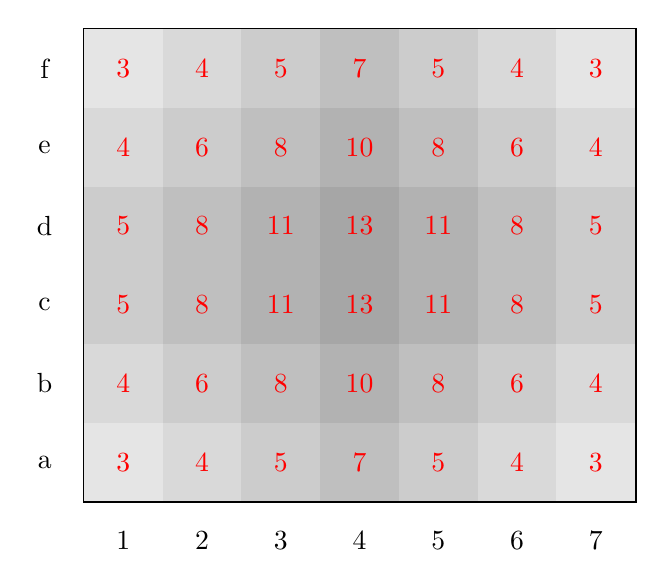
\begin{tikzpicture}[scale=1]
		% Zeichne das Gitter mit einheitlicher Linienstärke
		\foreach \x in {0,1,2,3,4,5,6} {
		\foreach \y in {0,1,2,3,4,5} {
			\draw[line width=1pt] (\x,\y) rectangle ++(1,1);
		}
	}
	
	% Beschriftung für Spalten (1-7)
	\foreach \x [count=\i from 1] in {1,2,3,4,5,6,7} {
		\node at (\i-0.5,-0.5) {\x};
	}
	
	% Beschriftung für Zeilen (a-f)
	\foreach \y [count=\j from 1] in {a,b,c,d,e,f} {
		\node at (-0.5,\j-0.5) {\y};
	}
		
		% Zahlen aus der Tabelle in die Felder einfügen und die Felder einfärben
		% Zeile 0
		\fill[gray!20] (0,5) rectangle ++(1,1); \node[red] at (0.5,5.5) {3};
		\fill[gray!30] (1,5) rectangle ++(1,1); \node[red] at (1.5,5.5) {4};
		\fill[gray!40] (2,5) rectangle ++(1,1); \node[red] at (2.5,5.5) {5};
		\fill[gray!50] (3,5) rectangle ++(1,1); \node[red] at (3.5,5.5) {7};
		\fill[gray!40] (4,5) rectangle ++(1,1); \node[red] at (4.5,5.5) {5};
		\fill[gray!30] (5,5) rectangle ++(1,1); \node[red] at (5.5,5.5) {4};
		\fill[gray!20] (6,5) rectangle ++(1,1); \node[red] at (6.5,5.5) {3};
		
		% Zeile 1
		\fill[gray!30] (0,4) rectangle ++(1,1); \node[red] at (0.5,4.5) {4};
		\fill[gray!40] (1,4) rectangle ++(1,1); \node[red] at (1.5,4.5) {6};
		\fill[gray!50] (2,4) rectangle ++(1,1); \node[red] at (2.5,4.5) {8};
		\fill[gray!60] (3,4) rectangle ++(1,1); \node[red] at (3.5,4.5) {10};
		\fill[gray!50] (4,4) rectangle ++(1,1); \node[red] at (4.5,4.5) {8};
		\fill[gray!40] (5,4) rectangle ++(1,1); \node[red] at (5.5,4.5) {6};
		\fill[gray!30] (6,4) rectangle ++(1,1); \node[red] at (6.5,4.5) {4};
		
		% Zeile 2
		\fill[gray!40] (0,3) rectangle ++(1,1); \node[red] at (0.5,3.5) {5};
		\fill[gray!50] (1,3) rectangle ++(1,1); \node[red] at (1.5,3.5) {8};
		\fill[gray!60] (2,3) rectangle ++(1,1); \node[red] at (2.5,3.5) {11};
		\fill[gray!70] (3,3) rectangle ++(1,1); \node[red] at (3.5,3.5) {13};
		\fill[gray!60] (4,3) rectangle ++(1,1); \node[red] at (4.5,3.5) {11};
		\fill[gray!50] (5,3) rectangle ++(1,1); \node[red] at (5.5,3.5) {8};
		\fill[gray!40] (6,3) rectangle ++(1,1); \node[red] at (6.5,3.5) {5};
		
		% Zeile 3
		\fill[gray!40] (0,2) rectangle ++(1,1); \node[red] at (0.5,2.5) {5};
		\fill[gray!50] (1,2) rectangle ++(1,1); \node[red] at (1.5,2.5) {8};
		\fill[gray!60] (2,2) rectangle ++(1,1); \node[red] at (2.5,2.5) {11};
		\fill[gray!70] (3,2) rectangle ++(1,1); \node[red] at (3.5,2.5) {13};
		\fill[gray!60] (4,2) rectangle ++(1,1); \node[red] at (4.5,2.5) {11};
		\fill[gray!50] (5,2) rectangle ++(1,1); \node[red] at (5.5,2.5) {8};
		\fill[gray!40] (6,2) rectangle ++(1,1); \node[red] at (6.5,2.5) {5};
		
		% Zeile 4
		\fill[gray!30] (0,1) rectangle ++(1,1); \node[red] at (0.5,1.5) {4};
		\fill[gray!40] (1,1) rectangle ++(1,1); \node[red] at (1.5,1.5) {6};
		\fill[gray!50] (2,1) rectangle ++(1,1); \node[red] at (2.5,1.5) {8};
		\fill[gray!60] (3,1) rectangle ++(1,1); \node[red] at (3.5,1.5) {10};
		\fill[gray!50] (4,1) rectangle ++(1,1); \node[red] at (4.5,1.5) {8};
		\fill[gray!40] (5,1) rectangle ++(1,1); \node[red] at (5.5,1.5) {6};
		\fill[gray!30] (6,1) rectangle ++(1,1); \node[red] at (6.5,1.5) {4};
		
		% Zeile 5
		\fill[gray!20] (0,0) rectangle ++(1,1); \node[red] at (0.5,0.5) {3};
		\fill[gray!30] (1,0) rectangle ++(1,1); \node[red] at (1.5,0.5) {4};
		\fill[gray!40] (2,0) rectangle ++(1,1); \node[red] at (2.5,0.5) {5};
		\fill[gray!50] (3,0) rectangle ++(1,1); \node[red] at (3.5,0.5) {7};
		\fill[gray!40] (4,0) rectangle ++(1,1); \node[red] at (4.5,0.5) {5};
		\fill[gray!30] (5,0) rectangle ++(1,1); \node[red] at (5.5,0.5) {4};
		\fill[gray!20] (6,0) rectangle ++(1,1); \node[red] at (6.5,0.5) {3};
		
	\end{tikzpicture}
	\caption{Bewertungstabelle: mögliche Anzahl an Vierer-Reihen}

\end{figure}
	
	\subsection*{Erklärung der Werte:}
	\textbf{Zentrum des Spielfelds:} Die Felder im Zentrum (insbesondere Spalte 4 und die Zeilen neben dran 3 und 5) haben die höchsten Werte, da sie Teil mehrerer potenzieller Viererreihen sein können – sowohl horizontal, vertikal als auch diagonal. Das erklärt, warum das Feld in Spalte 4, Zeilen c und d, den maximalen Wert von 13 besitzt.\\
	
	\textbf{Ränder des Spielfelds:} Die Felder am Rand (also die ersten und siebten Spalten sowie die Reihen a und f) zeigen deutlich niedrigere Werte. Das liegt daran, dass sie weniger Gewinnlinien bieten. Ein Randfeld kann höchstens Teil einer horizontalen und einer diagonalen Viererreihe sein, weshalb dort oft Werte von 3 oder 4 zu finden sind.
	
	\subsection*{Strategische Bedeutung:}
	Die zentralen Felder sind besonders wichtig, weil sie viele Optionen bieten, um eine Viererreihe zu vervollständigen. Deshalb ist es entscheidend, die mittleren Spalten – vor allem Spalte 4 sowie die angrenzenden Spalten 3 und 5 – im Auge zu behalten. Diese Kontrolle kann den Unterschied im Spiel ausmachen.
	Im Gegensatz dazu haben die Randfelder weniger Einfluss auf den Verlauf des Spiels. Sie werden oft hauptsächlich defensiv genutzt oder um den Gegner zu bestimmten Zügen zu zwingen.
	
	
\section{Entwicklung von Algorithmen}
In diesem Abschnitt werden verschiedene Algorithmen vorgestellt, die in unserem Projekt Anwendung finden können. Jeder Algorithmus wird zunächst in seinen Grundzügen erklärt, gefolgt von einer kritischen Bewertung zur Realisierung.
	
\subsection{MinMax-Algorithmus}

Die Minimax-Strategie ist ein grundlegender Algorithmus zur Entscheidungsfindung in Nullsummenspielen wie 4Gewinnt. Dieser Ansatz wird verwendet, um optimale Züge für einen Spieler zu finden, indem sowohl die eigenen Möglichkeiten als auch die möglichen Gegenreaktionen des Gegners analysiert werden. In diesem Kapitel wird die Funktionsweise der Minimax-Strategie im Kontext von 4Gewinnt betrachtet.

\subsection*{Grundprinzip der Minimax-Strategie}

Der Minimax-Algorithmus basiert auf der Idee, den eigenen Vorteil zu maximieren, während man gleichzeitig den Nutzen des Gegners minimiert. In einem Spielbaum, der alle möglichen Züge und die entsprechenden Reaktionen darstellt, sucht der Algorithmus nach dem besten Zug, indem er die Ergebnisse aller möglichen Entscheidungen bis zu einer bestimmten Tiefe analysiert.

In der Spieltheorie versteht man unter einem Spielbaum einen gerichteten Graphen ohne Zyklen, dessen Knoten die verschiedenen Spielstände darstellen. Dabei kann es vorkommen, dass derselbe Spielstand an mehreren Stellen im Baum auftaucht. Jeder Knoten zeigt auch an, welcher Spieler gerade am Zug ist. Der Spieler hat die Wahl, eine der möglichen Aktionen zu wählen, die durch die Kanten des Graphen repräsentiert werden.

Jeder Zustand im Baum ist entweder ein Endzustand oder hat eine Reihe von möglichen Folgepositionen, die durch die Züge im nächsten Spielzug erreicht werden können.

Die Bewertung der Spielstände erfolgt mithilfe einer Heuristik, die den Wert eines bestimmten Zustands quantifiziert. Bei 4Gewinnt könnte eine einfache Heuristik zum Beispiel folgende Aspekte berücksichtigen:

\begin{itemize}
	\item Gewonnene Spiele: Ein Zustand, in dem ein Spieler vier Steine in einer Reihe hat, hat den höchsten Wert.
	\item Blockierte Gewinnchancen: Züge, die verhindern, dass der Gegner vier in einer Reihe erreicht, sind besonders wertvoll.
	\item Teilweise vervollständigte Reihen: Zustände, in denen drei oder zwei verbundene Steine existieren, sind wertvoller als isolierte Steine.
\end{itemize}

Der Algorithmus berechnet mögliche Züge und bewertet sie rückwärts ausgehend von den möglichen Endzuständen.

In 4Gewinnt gibt es zwei Spieler:

\begin{itemize}
	\item Der Maximierer versucht, den eigenen Nutzen zu maximieren (z. B. Spieler 1).
	\item Der Minimierer versucht, den Nutzen des Gegners zu minimieren (z. B. Spieler 2).
\end{itemize}

Bei jedem Zug wechselt die Rolle zwischen Maximierer und Minimierer. Der Algorithmus wechselt daher bei jedem Ebenenwechsel zwischen der Maximierung und Minimierung der Heuristikwerte \autocites{krusenotto_anwendungsbeispiel_2016}.

\section*{Beispiel: Minimax-Suchbaum}

Im Folgenden wird ein einfacher Suchbaum dargestellt, der die Funktionsweise des Minimax-Algorithmus illustriert. Der Baum hat eine Tiefe von 4 (eine Max-Ebene und eine Min-Ebene).

\begin{figure}[H]
	\centering
	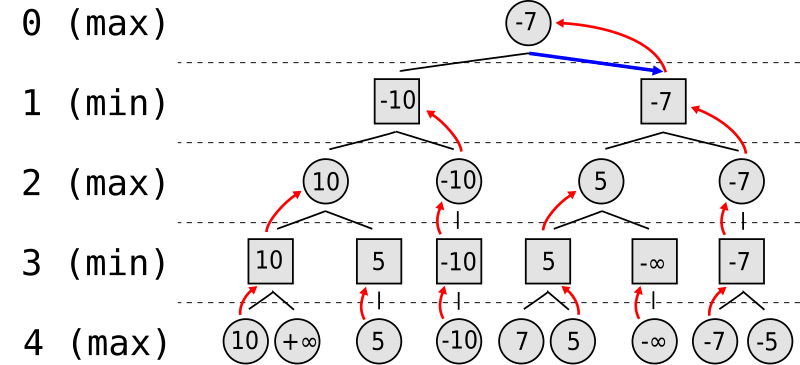
\includegraphics[width=0.7\linewidth]{images/Minimax.svg}
	\caption[Minimax-Suchbaum \autocite{Wikipedia:Minimax}]{Minimax-Suchbaum mit einer Tiefe von 4}
\end{figure}

\subsection*{Erklärung des Suchbaums}

Der Suchbaum in Abbildung \ref{fig:minimax} zeigt die Schritte des Minimax-Algorithmus:

\begin{enumerate}
	\item \textbf{Blattebene:} Die unterste Ebene enthält die Bewertungen der möglichen Endzustände aus Sicht des Max-Spielers. Diese Werte könnten durch eine Bewertungsfunktion ermittelt worden sein.

	\item \textbf{Min-Ebene:} Der Min-Spieler versucht, die Bewertung zu minimieren. Für jeden Min-Knoten wird der niedrigste Wert seiner Kindknoten ausgewählt:
	\begin{itemize}
		\item z.B. der linke äußere Min-Knoten wählt $\min(10, unendlich) = 10$.
	\end{itemize}
	
	\item \textbf{Max-Ebene:} Der Max-Spieler versucht, die Bewertung zu maximieren. Der Max-Knoten wählt den höchsten Wert aus den zurückgegebenen Bewertungen der Min-Knoten:
	\begin{itemize}
		\item z.B. Der linkere äußere Max-Knoten wählt $\max(10, 5) = 10$.
	\end{itemize}
\end{enumerate}

\subsection*{Optimale Entscheidung:}

Der optimale Zug für Max ist die rechte Verzweigung, die zum Wert -7 führt. Obwohl beide Optionen zu negativen Werten führen (-10 auf der linken Seite und -7 auf der rechten Seite), wählt Max den größeren der beiden Werte, also -7. Dies ist die beste Entscheidung für Max unter der Annahme, dass der Gegenspieler (Min) optimal spielt. Der rote Pfeil im Spielbaum zeigt genau diesen optimalen Entscheidungspfad an.

\subsection{AlphaBeta-Algorithmus}

er Alpha-Beta-Algorithmus ist eine cleverere Variante des Minimax-Algorithmus, die dessen Leistung deutlich verbessert. Er arbeitet so, dass er bestimmte Spielzüge, die für die finale Entscheidung unwichtig sind, einfach ignoriert. Dadurch kann der Alpha-Beta-Algorithmus die Anzahl der Knoten, die im Spielbaum bewertet werden müssen, erheblich reduzieren. Das ist besonders hilfreich in ressourcenbegrenzten Umgebungen, wie zum Beispiel bei einem LEGO Spike Roboter, der nur begrenzte Rechenleistung hat.

Obwohl der Alpha-Beta-Algorithmus die gleichen Berechnungen wie der Minimax-Algorithmus anstellt, nutzt er zusätzlich zwei Parameter, Alpha und Beta. Diese helfen, überflüssige Berechnungen zu vermeiden und machen den Prozess effizienter:

\begin{itemize}
	\item \textbf{Alpha}: Der aktuelle maximale Wert, den der Maximierer sicher erreichen kann.
	\item \textbf{Beta}: Der aktuelle minimale Wert, den der Minimierer sicher erreichen kann.
\end{itemize}

Während der Spielbaum durchgegangen werden Äste abgeschnitten, welche für die endgültige Entscheidung irrelevant sind – das nennt man Pruning. Das passiert in den folgenden Fällen:
\begin{itemize}
	\item Ein Knoten einen Wert liefert, der schlechter ist als der bisher bekannte Alpha-Wert für den Maximierer.
	\item Ein Knoten einen Wert liefert, der schlechter ist als der bisher bekannte Beta-Wert für den Minimierer.
\end{itemize}

Die Anwendung des Alpha-Beta-Algorithmus auf 4Gewinnt bietet mehrere Vorteile:
\begin{itemize}
	\item \textbf{Effizienz}: Der Algorithmus reduziert die Anzahl der Knoten, die bewertet werden müssen, erheblich. Dies ermöglicht die Analyse tieferer Spielbäume mit derselben Rechenleistung.
	\item \textbf{Flexibilität}: Der Algorithmus lässt sich ganz einfach an die speziellen Bewertungsfunktionen von 4Gewinnt anpassen. So kann er beispielsweise Reihen, Spalten und Diagonalen bewerten.
	\item \textbf{Optimierung für begrenzte Ressourcen}: Ein LEGO Spike Roboter hat begrenzte Rechen- und Speicherkapazitäten. Der Alpha-Beta-Algorithmus ermöglicht es, in Echtzeit Züge zu berechnen, ohne den Roboter zu überlasten \autocites{monien_alphabeta-algorithmus_2008}.
\end{itemize}

\section*{Beispiel: Alpha-Beta-Suchbaum}

Im Folgenden wird ein einfacher Suchbaum dargestellt, der die Funktionsweise des Alpha-Beta-Algorithmus illustriert. Der Baum zeigt, wie bestimmte Zweige (\textit{Pruning}) abgeschnitten werden, um die Effizienz zu erhöhen.

\begin{figure}[H]
	\centering
	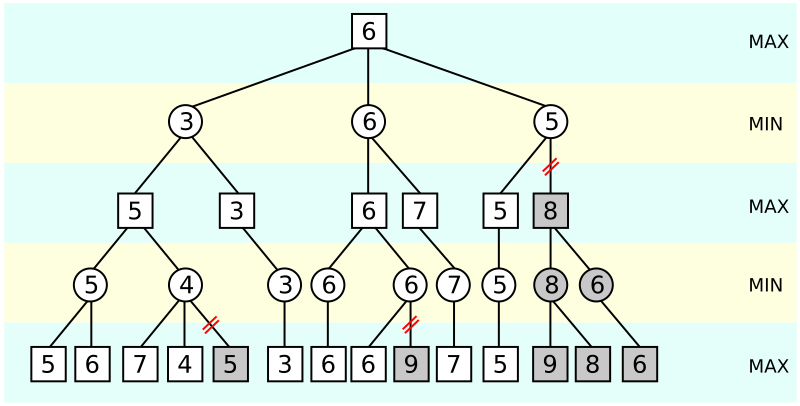
\includegraphics[width=0.7\linewidth]{images/AB_pruning.svg}
	\caption[Alpha-Beta-Suchbaum \autocite{Wikipedia:AlphaBeta}{Alpha-Beta-Suchbaum mit einer Tiefe von 4}
	\label{fig:abpruning}
\end{figure}

\subsection*{Erklärung des Suchbaums}

\begin{enumerate}
\item \textbf{Blattebene:} Die unterste Ebene enthält die Bewertungen der möglichen Endzustände aus Sicht des Max-Spielers. Diese Werte repräsentieren die Spielsituationen.
	\item \textbf{Min-Ebene:} Der Min-Spieler wählt den minimalen Wert seiner Kindknoten. Durch Alpha-Beta-Schnitte (mit $\times$ markiert) werden einige Äste nicht weiter untersucht, da sie das Endergebnis nicht mehr beeinflussen können.
\begin{itemize}
\item z.B. der linke Min-Knoten wählt $\min(5, 6) = 5$. Der nächste Min-Knoten bricht nach dem Wert von 4 ab, da die Zahl von 5 schon unterschritten wird und somit keinen Einfluss auf den nächsten Max-Knoten mehr hat.
    \end{itemize}
	\item \textbf{Max-Ebene:} Der Max-Spieler wählt den maximalen Wert. Auch hier werden durch Alpha-Beta-Schnitte (mit $\times$ markiert) einige Äste nicht weiter untersucht, da sie das Endergebnis nicht mehr beeinflussen können.

	\begin{itemize}
\item z.B der linke Max-Knoten wählt $\max(5, 4) = 5$


	\end{itemize}
	
\end{enumerate}

\subsection*{Optimale Entscheidung}
Schließlich wählt der Wurzelknoten (MAX) den Wert 6 als Maximum der drei darunterliegenden Werte. Durch Alpha-Beta-Pruning werden einige Zweige nicht weiter untersucht, da sie das Endergebnis nicht mehr beeinflussen können, was die Effizienz des Algorithmus erhöht. Der optimale Spielwert beträgt 6 und wird über den mittleren Pfad erreicht.

\subsection*{Vorteile des Alpha-Beta-Algorithmus}

Durch das Alpha-Beta-Pruning werden unnötige Berechnungen vermieden:
\begin{itemize}
	\item Der Algorithmus durchsucht nur jene Zweige, die potenziell zu besseren Ergebnissen führen.
	\item Dies erhöht die Effizienz und ermöglicht es, tiefere Suchbäume mit derselben Rechenleistung zu analysieren\autocites{monien_alphabeta-algorithmus_2008}.
\end{itemize}